\paragraph{Task dependences}

By creating tasks instead of sections, each thread can execute any task as long as its input is ready. Since the internal scheduler decides how to manipulate the execution of tasks, there is a useful \textbf{clause to indicate a dependency between tasks}.
\marginpar{
    \href{https://www.openmp.org/spec-html/5.0/openmpsu99.html} {Doc. \faIcon{book}}
}
\begin{openmpbox}[: \texttt{depend}]
    \begin{lstlisting}[language=C++, mathescape=true]
#pragma omp task depend($\emph{dependence-type}$: variable)\end{lstlisting}
    The \texttt{depend} clause enforces additional constraints on the scheduling of tasks or loop iterations. These constraints establish dependencies only between sibling tasks or between loop iterations.

    The \emph{dependence-type} can be \texttt{in} or \texttt{out}.
\end{openmpbox}

\noindent
In addition to the depend clause, we can also use the priority clause to hint that more important tasks should be executed more frequently.

\highspace
The \texttt{priority} clause is a \textbf{hint for the priority of the generated task}. The priority-value is a \textbf{non-negative integer expression} that provides a hint for task execution order. Among all tasks ready to be executed, \textbf{higher priority tasks} (those with a higher numerical value in the priority clause expression) \textbf{are recommended to execute before lower priority ones}. The \textbf{default} priority-value when no priority clause is specified \textbf{is zero} (the \emph{lowest priority}).

\highspace
\textbf{If a value is specified in the priority clause that is higher than the \emph{max-task-priority-var}} ICV (internal control variables) then the implementation will \textbf{use the value of that ICV}. A program that relies on task execution order being determined by this priority-value may have unspecified behavior.
\begin{itemize}
    \item The \texttt{omp\_get\_max\_task\_priority} routine returns the \textbf{maximum value that can be specified in the \texttt{priority} clause}.
    \marginpar{
        \href{https://www.openmp.org/spec-html/5.0/openmpsu151.html\#x188-8880003.2.42} {Doc. \faIcon{book}}
    }
    \begin{openmpbox}[: \texttt{omp\_get\_max\_task\_priority}]
        \begin{lstlisting}[language=C++]
int omp_get_max_task_priority()\end{lstlisting}
    \end{openmpbox}

    \item The \texttt{OMP\_MAX\_TASK\_PRIORITY} environment variable \textbf{controls the use of task priorities} by setting the initial value of the \emph{max-task-priority-var} ICV. The value of this environment variable must be a non-negative integer.\marginpar{
        \href{https://www.openmp.org/spec-html/5.0/openmpse64.html\#x303-20810006.16} {Doc. \faIcon{book}}
    }
\end{itemize}

\begin{flushleft}
    \textcolor{Red2}{\faIcon{exclamation-triangle} \textbf{Possible overhead}}
\end{flushleft}
The task in general, but especially the \textbf{dependencies between tasks, can introduce overhead and reduce performance}.

\newpage

\begin{examplebox}[: dependences]
    Let the following parallel code:
    \begin{lstlisting}[language=C++, mathescape=true]
#pragma omp parallel default(none) \
                     shared(fp_read) \
                     shared(n_io_chunks) \
                     shared(n_work_chunks) \
                     shared(a, b, c) \
                     shared(status_read, status_processing) \
                     shared(status_postprocessing)
{
    #pragma omp single nowait
    {
        for(int64_t i = 0; i < n_io_chunks; ++i) {
            #pragma omp task depend(out: status_read[i]) \
                             priority(20)
            {
                (void) read_input(
                    fp_read, i, a, b, &status_read[i]
                );
            } // End of task reading in a chunk of data

            #pragma omp task depend(in: status_read[i]) \
                        depend(out: status_processing[i]) \
                        priority(10)
            {
                (void) compute_results(
                    i, n_work_chunks, a, b, c,
                    &status_processing[i]
                );
            } // End of task performing the computations

            #pragma omp task depend(in: status_processing[i])
                             priority(5)
            {
                (void) postprocess_results(
                    i, n_work_chunks, c,
                    &status_postprocessing[i]
                );
            } // End of task postprocessing the results
        } // End of for-loop
    } // End of single region
} // End of parallel region
    \end{lstlisting}
    \begin{itemize}
        \item Row 11. We are going to process \texttt{n\_io\_chunks} of data.
        \item Rows 12, 20. Refer to read and are compute dependence.
        \item Rows 21, 30. Refer to compute and are postprocess dependence.
    \end{itemize}
    \newpage
    A possible order of execution if we consider 3 threads is:
    \begin{center}
        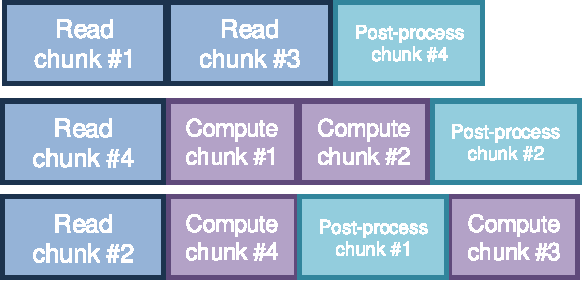
\includegraphics[width=.6\textwidth]{img/task-dependence-1.pdf}
    \end{center}
    As long as the dependencies are respected, the loop iterations can be executed in any order. No explicit \texttt{flush} (page \hyperlink{openmp: flush}{\hypergetpageref{openmp: flush}}) are required because it is implied before and after every task.
\end{examplebox}

\begin{flushleft}
    \textcolor{Green3}{\faIcon{question-circle} \textbf{Custom number of iterations}}
\end{flushleft}
\textbf{Each task gets assigned a number of iterations which is the minimum between \texttt{grainsize} and the total number of iterations}.

\highspace
If a \texttt{grainsize} clause is present, the number of logical iterations assigned to each generated task is greater than or equal to the minimum of the value of the \texttt{\emph{grain-size}} expression and the number of logical iterations, but less than two times the value of the \texttt{\emph{grain-size}} expression.

\highspace
If the \texttt{grainsize} clause has the \texttt{\emph{strict}} modifier, the number of logical iterations assigned to each generated task is equal to the value of the \texttt{\emph{grain-size}} expression, except for the generated task that contains the sequentially last iteration, which may have fewer iterations. The parameter of the \texttt{grainsize} clause must be a positive integer expression.
\marginpar{
    \href{https://www.openmp.org/spec-html/5.1/openmpsu55.html} {Doc. \faIcon{book}}
}
\begin{openmpbox}[: \texttt{pragma omp taskloop grainsize}]
    \begin{lstlisting}[language=C++, mathescape=true]
#pragma omp taskloop grainsize($\emph{[strict] grain-size}$)\end{lstlisting}
\end{openmpbox}

\newpage

\begin{flushleft}
    \textcolor{Green3}{\faIcon{question-circle} \textbf{Number of created tasks}}
\end{flushleft}
\textbf{To keep the number of created tasks low, the clause \texttt{num\_tasks} sets the number of tasks that the runtime system can generate}.

\highspace
If \texttt{num\_tasks} is specified, the \texttt{taskloop} construct creates as many tasks as the minimum of the \texttt{\emph{num-tasks}} expression and the number of logical iterations. Each task must have at least one logical iteration. The parameter of the \texttt{num\_tasks} clause must be a positive integer expression.

\highspace
If the \texttt{num\_tasks} clause has the \texttt{\emph{strict}} modifier for a task loop with $N$ logical iterations, the logical iterations are partitioned in a balanced manner and each partition is assigned, in order, to a generated task. The partition size is $\left\lceil\left\lceil \dfrac{N}{\texttt{\emph{num-tasks}}} \right\rceil \right\rceil$ until the number of remaining iterations divides the number of remaining tasks evenly, at which point the partition size becomes $\left\lfloor\left\lfloor \dfrac{N}{\texttt{\emph{num-tasks}}} \right\rfloor\right\rfloor$.
\marginpar{
    \href{https://www.openmp.org/spec-html/5.1/openmpsu55.html} {Doc. \faIcon{book}}
}
\begin{openmpbox}[: \texttt{pragma omp taskloop num\_tasks}]
    \begin{lstlisting}[language=C++, mathescape=true]
#pragma omp taskloop num_tasks($\emph{[strict] num-tasks}$)\end{lstlisting}
\end{openmpbox}

\highspace
\textbf{If neither a \texttt{grainsize} nor \texttt{num\_tasks} clause is present, the number of loop tasks generated and the number of logical iterations assigned to these tasks is implementation defined.}